\documentclass[a4paper]{article}

\usepackage{color}
\usepackage{url}
\usepackage[T2A]{fontenc}
\usepackage[utf8]{inputenc} 
\usepackage{graphicx}


\usepackage{blindtext}
\usepackage{enumitem}
\usepackage{xcolor}

\usepackage[english,serbian]{babel}

\usepackage[unicode]{hyperref}
\hypersetup{colorlinks,citecolor=green,filecolor=green,linkcolor=blue,urlcolor=blue}


\newtheorem{primer}{Primer}[section]

\begin{document}

\title{Gordon Bel\\ \small{Seminarski rad u okviru kursa\\Tehničko i naučno pisanje\\ Matematički fakultet}}

\author{Darija Eremija, Katarina Kilibarda, Dejan Živković, Anja Jovanović\\ darijae99@gmail.com, kaja.kilibarda@gmail.com, \\ dejan199930@gmail.com, jovanovic.anja99@gmail.com}
\date{10.~novembar 2019.}
\maketitle

\abstract{
Č. Gordon Bel (engl. C. Gordon Bell; Kirksvil 19. avgust 1934) je Američki inženjer elektrotehnike i rukovodilac. Zaposlen u korporaciji digitalne opreme(engl. Digital Equipment Corporation) 1960-1966,Bel je dizajnirao nekoliko njihovih PDP mašina, a kasnije je postao potpredsednik inžinjeringa 1972-1983, nadgledajući razvoj VAKS-a.  Belova kasnija karijera uključuje preduzetnika, investitora, pomoćnika direktora NSF-a za računarstvo i informacionu nauku i inženjerstvo 1986-1987, i emeritus istraživača u Majkrosoft Risrč-u, 1995–2015.

\tableofcontents


\newpage

\begin{tabular}{|c|l|}

\hline
\multicolumn{2}{|c|}{Gordon Bel} \tabularnewline
\hline
\multicolumn{2}{|c|}{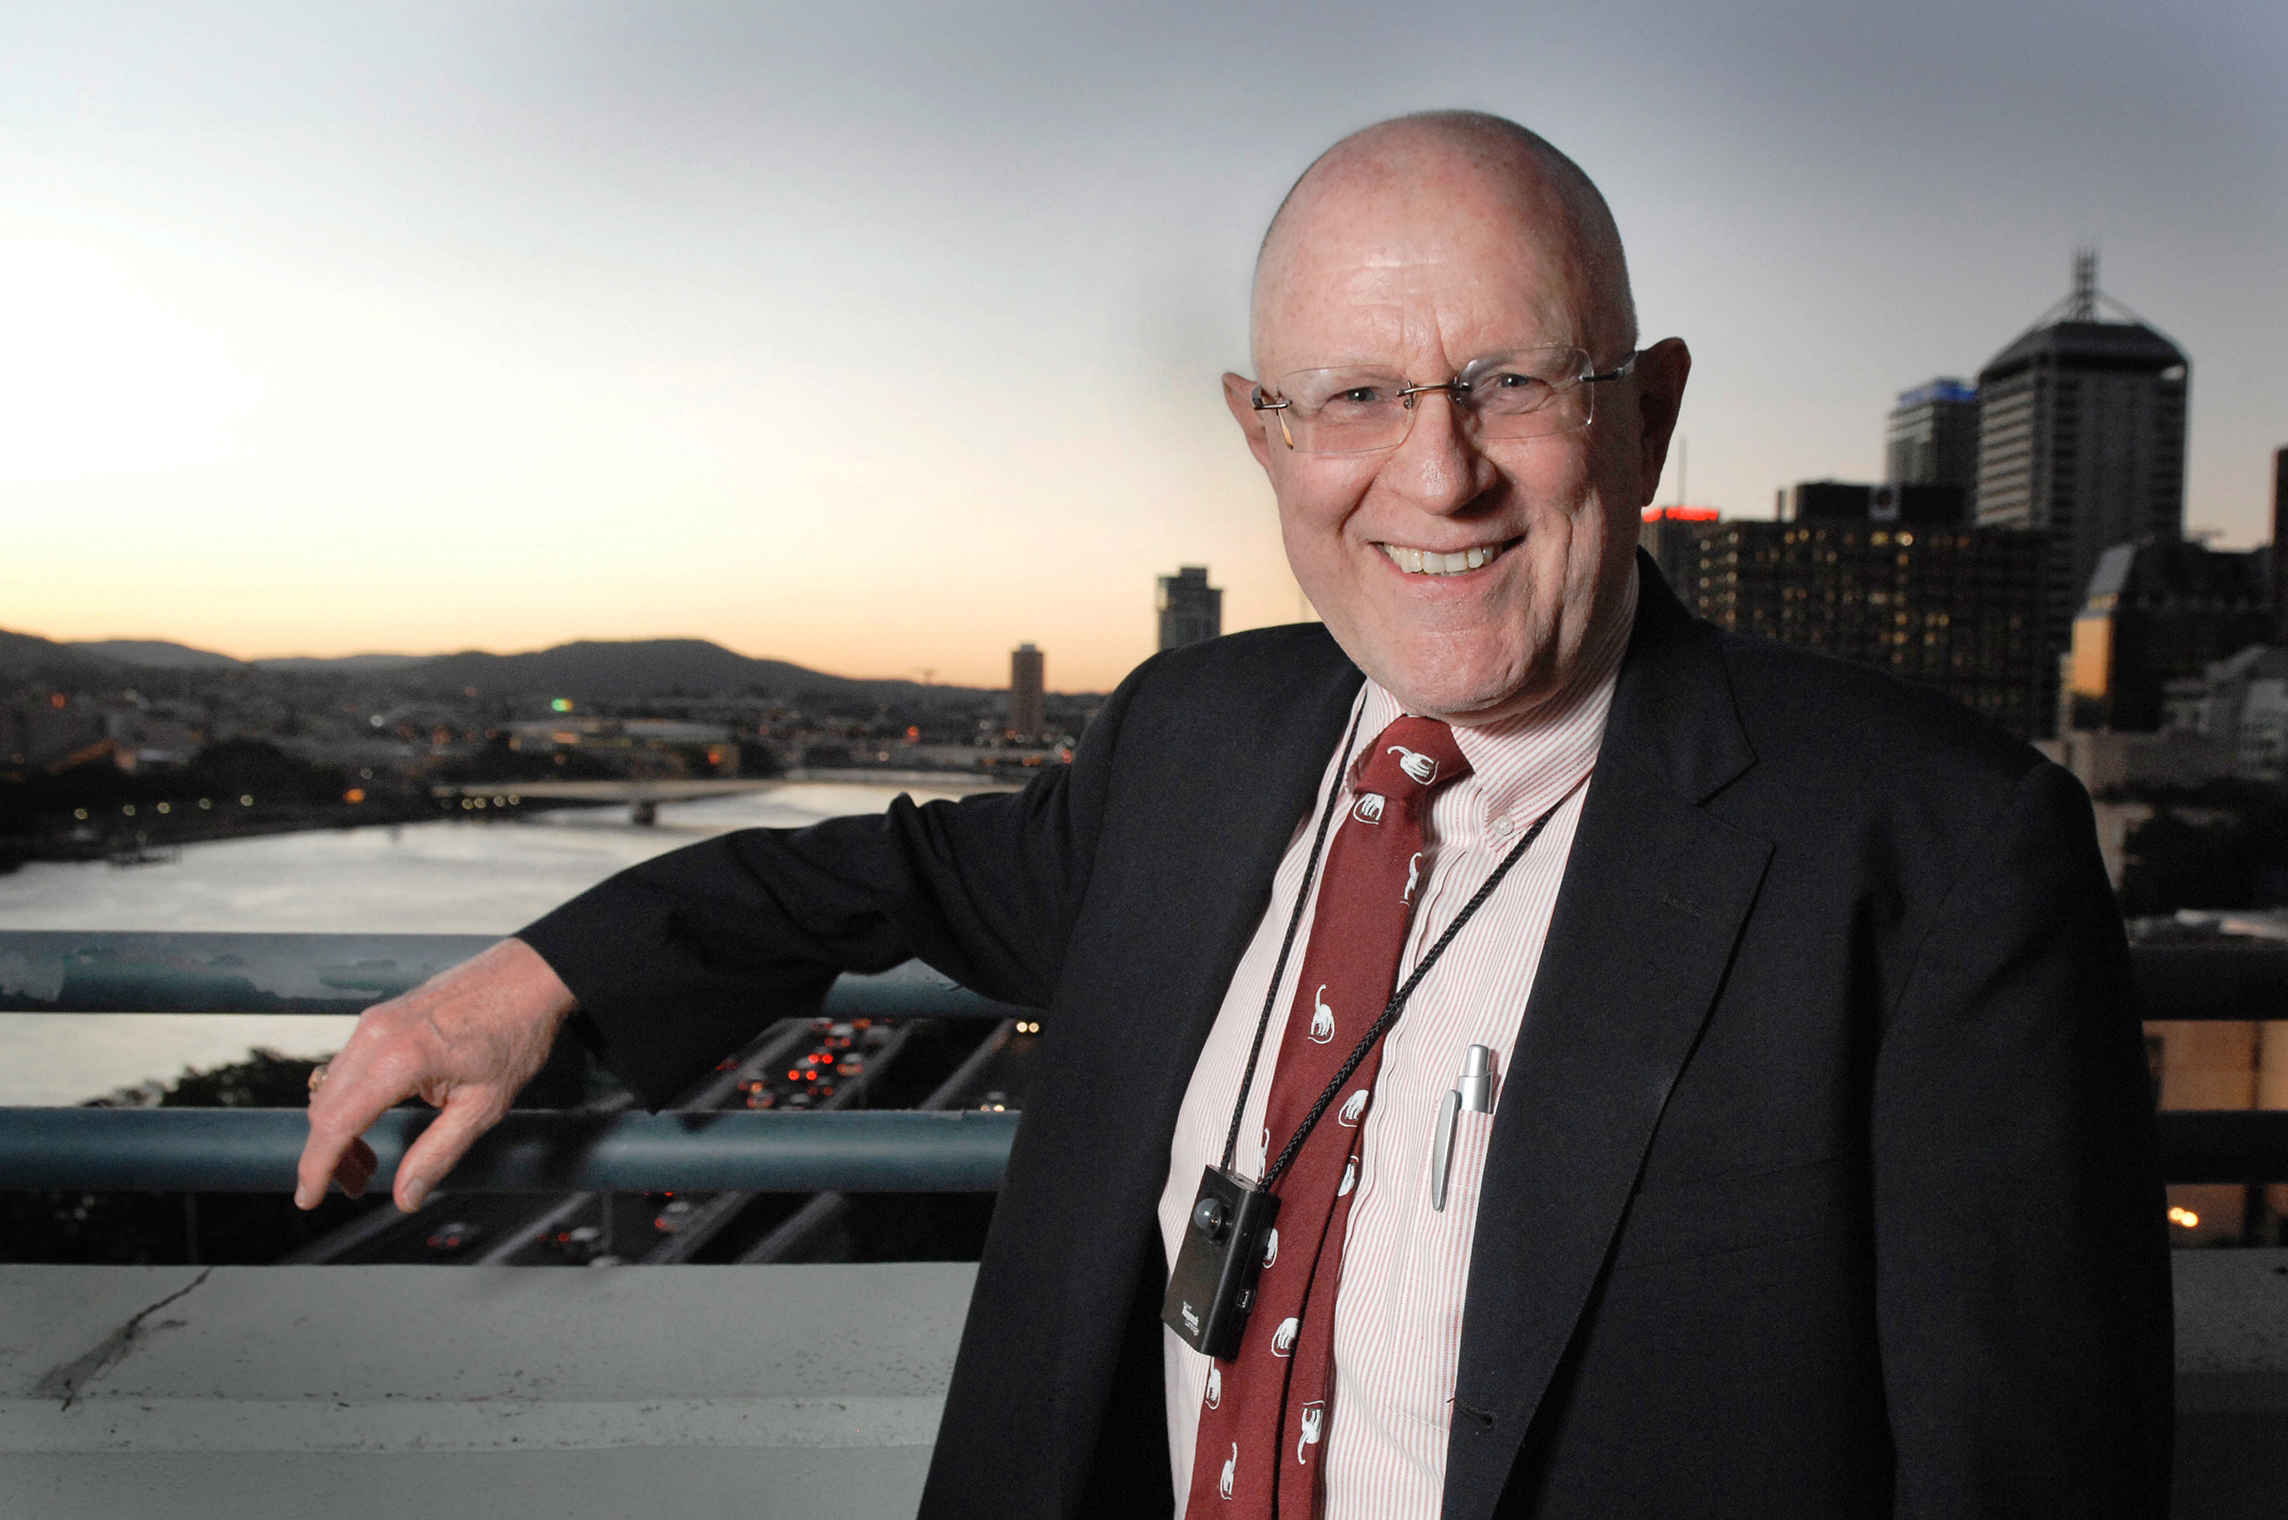
\includegraphics[width=260px,height=180px]{Gordon_Bell.jpg}} \\
\hline
Datum rođenja & 19.avgust 1934 \\
\hline
Mesto rođenja & Kirksvil,Sjedinjene Američke Države \\
\hline
Škola & Massachusetts Institute of Technology \\
\hline
\end{tabular}

\section{Rani život i edukacija}
\label{sec:uvod}
Čester Gordon Bel je rođen u Kirksvilu, Misuri. Odrastao je pomažući porodičnom preduzeću Bel Elektrik(engl. Bell Electric) popravljajući uređaje i ožičavajući domove\cite{bel1}.

Bel je postao diplomirani inženjer (1956) i magistar (1957) elektrotehnike sa MIT-a. Potom je otišao na Tehnološki univerzitet Novi Južni Vels (sada UNSV) u Australiju na Fulbright stipendiju, gde je predavao časove računarskog dizajna, programirao jedan od prvih računara koji je stigao u Australiju (zvan UTECOM, engleski Elektrik DEUCE) i objavio svoj prvi akademski rad. Vrativši se u Sjedinjene Američke Države, radio je u MIT Speech Computation Laboratory kod profesora Kena Stivensa, gde je napisao prvi program Analiza sinteze.

\section{Karijera}
\subsection{Korporacija digitalne opreme (Digital Equipment Corporation)}
\label{subsec:podnaslov1}

Osnivači korporacije digitalne opreme: Ken Olsen i Harlan Anderson regrutovali su ga za svoju novu kompaniju 1960. godine, gde je dizajnirao U/I (ulaz/izlaz) podsistem za programirani procesor podatka 1 (engl. Programmed Data Processor-1) , uključujući i prvi univerzalni asinhroni prijemnik-predajnik (engl. universal asynchronous receiver-transmitter). Bel je bio arhitekta podsistema programiranog procesora podatka 4 (engl. Programmed Data Processor-4) i podsistema programiranog procesora podatka 6 (engl. Programmed Data Processor-6). Drugi arhitektonski doprinosi bili su za podsistem programiranog procesora podatka 5 (engl. Programmed Data Processor-5) i podsistem programiranog procesora podatka 11 (engl. Programmed Data Processor-11) unibus i generalni registri arhitekture. \cite{bel2}

Nakon korporacije digitalne opreme, Bel je otišao na Univerzitet Karnegije Melon 1966. godine da predaje računarske nauke, ali se vratio u korporaciju digitalne opreme 1972. godine kao potpredsednik inženjerstva, gde je bio zadužen za VAKS (engl. VAX), najuspešniji računar korporacije digitalne opreme.

\subsection{Preduzetnik i savetnik za polise}
\label{subsec:podnaslov1}
Bel se povukao iz korporacije digitalne opreme 1983. zbog srčanog udara, ali ubrzo nakon je osnovao Enkore Kompjuter (engl. Encore Computer), jedan od prvih računara sa deljenom memorijom i sa više mikroprocesora koji su koristili strukturu keš memorije.

Tokom 1980-ih uključio se u javnu politiku, postajući prvi osnivajući pomoćnik direktora direkcije računara, informatike i inženjeringa (engl. computers and information science and engineering) i rukovodio je \-me\-đu\-re\-so\-rskom grupom koja je specificirala nacionalnu istraživačku i edukacionu mrežu (engl. national research and education network (NREN)).

Bel je takođe osnovao nagradu Gordon Bel 1987. (kojom upravljaju asocijacija za kompjuterske sisteme (engl. association for computing \-ma\-chi\-ne\-ry-ACM) i institut inženjera elektrotehnike i elektronike (IEEE)) da bi podstakao razvoj paralelne obrade. Prvu nagradu Gordon Bel osvojili su istraživači iz odeljenja za paralelnu obradu nacionalne laboratorije Sandia za rad urađen na hiperkubi 1000 (engl. nCUBE) 10 procesora.

Bio je član osnivača kompanije Ardent Kompjuter 1986. godine, postajući zamenik predsednika za istraživanje i razvoj 1988. godine, i ostao je sve dok se 1989. godine nije spojio sa Stellarom, da bi postao Stardent kompjuter.
\subsection{Majkrosoft istraživanje}
\label{subsec:podnaslov1}
Između 1991. i 1995. godine, Bel je savetovao Majkrosoft u naporima da pokrene istraživačku grupu, a zatim mu se u avgustu 1995. godine pridružio sa punim radnim vremenom, proučavajući teleprisutnost i srodne ideje. On je predmet eksperimenta za MajLajfBits (engl. MyLifeBits) projekat, eksperiment u beleženju života (nije isto što i životno blogiranje) i pokušaj ispunjenja Vanevar Bušove vizije o automatizovanom skladištu dokumenata, slika (uključujući i one snimljene automatski) i zvukovi koje je pojedinac doživeo tokom svog života, da im se može pristupiti brzo i lako. Zbog toga je Bel digitalizovao sve dokumente koje je pročitao ili proizveo, CD-ove, e-poštu i tako dalje. Nastavio je to da radi, prikupljajući pregledane veb stranice, razgovore putem telefona i trenutnih poruka i slično manje-više automatski.

Nakon korporacije digitalne opreme, Bel je otišao na Univerzitet Karnegije Melon 1966. godine da predaje \-ra\-ču\-na\-rske nauke, ali se vratio u korporaciju digitalne opreme 1972. godine kao potpredsednik inženjerstva, gde je bio zadužen za VAKS (engl. VAX), najuspešniji računar korporacije digitalne opreme.


\section{Počasti}	
\label{sec:termini_i_citiranje}

Bel je saradnik Američke Akademije Umetnosti i Nauka (1994),\cite{bel3} Američkog Udruženja za Unapređenje Nauke (1983), Asocijacije za \-Ra\-ču\-nar\-ske Mašine (1994), IEEE (1974), i član Nacionalne Akademije \-Inže\-njer\-stva (1977), Nacionalne Akademije Nauka (2007) i saradnik Australijske Akademije Tehnoloških Nauka i Inženjerstva (2009).

Takođe je član savetodavnog odbora TTI / Vangurd-a (engl. TTI/Va\-nguard) i bivši član sektorskog saveta za informacionu i komunikacionu tehnologiju australijske organizacije za naučno-industrijska istraživanja zajednice Komonvelth (engl. Commonwealth Scientific and Industrial Research Organisation) .

Bel je prvi dobitnik medalje IEEE Džon von Nejman, 1992. godine.\cite{bel4} Njegove ostale nagrade uključuju člana muzeja računarske istorije, počasnog doktora inžinjerstva od Vorcester politehničkog instituta (engl. Worcester Polytechnic Institute (WPI)), nagrade američke asocijacije za elektoniku (engl. American Electronics Association AeA ), nagrade za izuzetna tehnička dostignuća Vladimira Karapetofa Eta Kapa Nu i 1991. nacionalnog odličja za tehnologiju od predsednika Džordža H.V. Buša. \cite{bel5} Takođe je 2007. godine proglašen za eminentnog člana Eta Kapa Nu.

Godine 1993. Vorkester Politehnik Institut je proglasio Bela počasnim doktorom inžinjeringa, a 2010. godine Bel je primio dilomu počasnog doktora nauke i tehnologije sa Karnegi Melon Univerziteta. Univerzitet ga je prozvao "ocem mini-računara".

Bel je bio ko-osnivač Muzeja računara, u Bostonu, Masačusets, zajedno sa svojom ženom Gven Bel 1979. godine. Bio je član osnivačkog odbora naslednika Muzeja računara, Muzeja istorije računara,u Mauntin Vjuu, Kalifornija. Godine 2003. Bel je postao saradnik muzeja zbog svoje ključne uloge u revoluciji mini-računara i za doprinos kao arhitekta računara i preduzetnik.\cite{bel6} Priča o revoluciji muzeja počinje ranih 1970-ih sa Kenom Olsenom u Korporaciji Digital Ekvipment opisana je u Majkrosoftovom tehničkom izveštaju MCR-TP-2011-44, "Izvan Ormana: Muzej Ranih Godina Računara[x]*". \cite{bel7} Na njegovom veb sajtu \cite{bel8} nalazi se vremenska linija računanja istorijskih mašina, događaja i ljudi. Ona pokriva B.C. do danas.




\section{Belov zakon računarskih klasa}
\label{slike_i_tabele}

Belov zakon računarskih klasa \cite{bel9} je prvi put opisan 1972. godine sa pojavom nove klase mikroračunara niže cene zasnovane na mikroprocesoru. Uspostavljeni računari tržišne klase uvode se po stalnoj ceni s povećanjem funkcionalnosti i performansi. Napredak tehnologije u poluvodičima, skladištu, interfejsima i mrežama omogućava da se formira nova računarska klasa (platforma) svake decenije kako bi se zadovoljila nova potreba. Svaka nova klasa obično niže cene održava se kao kvazi nezavisna industrija (tržište). Klase uključuju: mejnfrejmove (1960-e), mini-računare (1970-e), umrežene radne stanice i lične računare (1980-e), strukturu pretraživača-veb-servera (1990-e), palm računarstvo (1995), veb usluge (2000-e), konvergenciju mobilnih telefona i računara (2003) i Bežične Senzorske Mreže poznatije kao motes (2004). Bel je predvideo da će se mreže za dom i telo formirati do 2010. godine.

\section{Knjige}
\label{sec:naslov1}

\begin{itemize}
\item (sa Alanom Njuelom) Računarske strukture: Literatura i Primeri (1971, ISBN 0-07-004357-4)
\item (sa C. Madžom i J. Mek Namarom) Računarsko inženjerstvo (1978, ISBN 0-932376-00-2)
\item (sa Danom Sjviorekom i Alanom Njuelom) Računarske strukture: Literatura i Primeri (1982, ISBN 0-07-057302-6)
\item (sa J. Mek Namarom) Visoko tehnološki poduhvati: Vodič za uspeh u preduzetništvu (1991, ISBN 0-201-56321-5)
\item (sa Džimom Gemelom) Celokupno podsećanje: Kako će E-Memorijska Revolucija promeniti sve (2009, ISBN 978-0-525-95134-6)
\item (sa Džimom Gemelom) Tvoj Otpremljeni život: Digitalni put ka boljem pamćenju, zdravlju i produktivnosti (2010, ISBN 978-0-452-29656-5)


\end{itemize} 

\addcontentsline{toc}{section}{Literatura}
\appendix
\bibliography{seminarski} 
\bibliographystyle{plain}

\appendix
\renewcommand{\refname}{Reference}
\begin{thebibliography}{9}
\bibitem{bel1} Gardner Hendri, Intervju (jun 23, 2005). \href{https://computerhistory.org/collections/accession/102702036}{"Bell (Gordon) Oral History"} . Broj reference: X3202.2006. Muzej računarske istorije. Pristupljeno 20.5.2011. 
\bibitem{bel2} Intervju arhiviran 2.4.2005. na \href{https://sr.wikipedia.org/wiki/Wayback_Machine}{Vejbek mašini} kustosa Davida K. Alisona, Nacionalni muzej američke istorije, SAD, 1995.
\bibitem{bel3}  "Book of Members, 1780-2010: Chapter B" (PDF). Američka akademija nauke i umetnosti. Pristupljeno 30.5.2011.
\bibitem{bel4} "IEEE John von Neumann Medal Recipients" (PDF). IEEE. Pristupljeno 31.12.2010.
\bibitem{bel5} \href{https://www.uspto.gov/learning-and-resources/ip-programs-and-awards/national-medal-technology-and-innovation-nmti}{ "The National Medal of Technology and Innovation Recipients - 1991 Laureates"} . Ured za patente i zaštitne znakove Sjedinjenih Država. Pristupljeno 31. decembra 2010. Godine 1991. nagrada se zvala Nacionalna medalja za tehnologiju.
\bibitem{bel6} "Gordon Bell". Muzej računarske istorije. Pristupljeno 23.5.2013.
\bibitem{bel7}  Bel, Gordon (4. april 2011.). \href{https://www.microsoft.com/en-us/research/publication/out-of-a-closet-the-early-years-of-years-of-the-computer-x-museums/}{"Out of a Closet: The Early Years of The Computer [x]* Museum"}. Majkrosoftov tehnički izveštaj MSR-TR-2011-44. Korporacija Majkrosoft. Pristupljeno 12.4.2011.
\bibitem{bel8} Bel, Gordon (20. april 2014). \href{https://gordonbell.azurewebsites.net/}{"Timeline of Computing History: Artifacts, Computers, Inventions, People, and Events --B.C. to 2014"} . Research.microsoft.com.
\bibitem{bel9}  Bel, G., "Bell’s Law for the Birth and Death of Computer Classes", Communications of the ACM, Januar 2008, tom 51, br. 1, pp 86–94. 
 

\end{thebibliography}

\section{Dodatna literatura}
\label{sec:naslov1}
\begin{itemize}
\item Vilkinson, Alek,\href{https://www.newyorker.com/magazine/2007/05/28/remember-this}{"Remember This?"}  Njujorker, 28. maj 2007., pp.38–44.

\end{itemize} 

\section{Spoljašnje veze}
\label{sec:naslov1}
\begin{itemize}
\item \href{https://web.archive.org/web/20050402125352/http://americanhistory.si.edu/collections/comphist/bell.htm}{Intervju} Intervju kustosa Davida K. Alisona, Nacionalni muzej američke istorije, SAD, 1995.
\item \href{https://www.cbsnews.com/video/a-stitch-in-time-recorded/?lumiereId=50022828&videoId=66c07162-8bdf-11e2-9400-029118418759&cbsId=2666250&site=cbsnews}{CBS večernje vesti video intervju}  na MyLifeBits projetku, 2007.

\end{itemize} 


\end{document}
